\documentclass[classe=$2^{de}$]{exercice}

\usepackage{tcolorbox}

\newcommand{\DotsCorrectionLong}{\makebox[8cm]{\dotfill}}

\title{Activité : intersection et union d'évènements}

\begin{document}

\maketitle

\begin{enumerate}
	\item Si $X$ et $Y$ sont des ensembles, on note :
	      \begin{itemize}
		      \item[] $\correctionDots{X ∩ Y}$ l'ensemble des éléments qui sont dans $X$ \textbf{ET} dans $Y$
		      \item[] $\correctionDots{X ∪ Y}$ l'ensemble des éléments qui sont dans $X$ \textbf{OU} dans $Y$
	      \end{itemize}

	      \begin{tcolorbox}
		      On considère la situation suivante :

		      On tire un premier jeton dans un sac contenant les jetons suivants :
		      \begin{center}
			      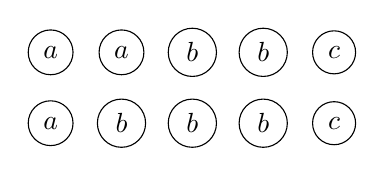
\begin{tikzpicture}[scale=0.9]
				      \foreach \l [count=\i] in {a,a,b,b,c} {
						      \node[circle,draw=black] at (\i,0) {$\l$};
					      }
				      \foreach \l [count=\i] in {a,b,b,b,c} {
						      \node[circle,draw=black] at (\i,-1) {$\l$};
					      }
			      \end{tikzpicture}
		      \end{center}

		      Puis on tire un deuxième jeton dans un sac contenant :
		      \begin{center}
			      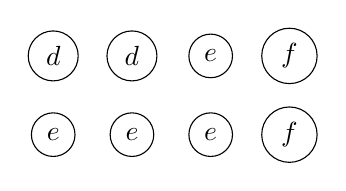
\begin{tikzpicture}
				      \foreach \l [count=\i] in {d,d,e,f} {
						      \node[circle,draw=black] at (\i,0) {$\l$};
					      }
				      \foreach \l [count=\i] in {e,e,e,f} {
						      \node[circle,draw=black] at (\i,-1) {$\l$};
					      }
			      \end{tikzpicture}
		      \end{center}
	      \end{tcolorbox}
	\item On considère les évènements suivants :
	      \begin{itemize}
		      \item[$X$] : Le premier jeton tiré est $a$
		      \item[$Y$] : Le deuxième jeton tiré est $d$
		      \item[$Z$] : Le premier jeton tiré est $c$
	      \end{itemize}

	      Décrire par une phrase les évènements :
	      \begin{itemize}
		      \item $X ∩ Y$ : \correctionOr{{\color{red}On a tiré les jetons $a$ et $d$}}{\DotsCorrectionLong}
		      \item $Y ∪ Z$ : \correctionOr{{\color{red}Le premier jeton est $c$, et le deuxième est $d$}}{\DotsCorrectionLong}
	      \end{itemize}
	\item Dessiner un arbre de probabilités correspondant à la situation de l'encadré :

	      \begin{center}
		      \begin{tikzpicture}[scale=0.9]
			      \coordinate (START) at (0,0);

			      \foreach \p/\l/\y in {A/a/3,B/b/0,C/c/-3} {
					      \node (\p) at (3,\y) {\correction{$\l$}};
					      \node (D) at (6,\y+1) {\correction{$d$}};
					      \node (E) at (6,\y) {\correction{$e$}};
					      \node (F) at (6,\y-1) {\correction{$f$}};
					      \ifdefined\makeCorrection
						      \draw (\p) -- node[above] {$1/4$} (D)
						      (\p) -- node[above right] {$1/2$} (E)
						      (\p) -- node[below] {$1/4$} (F);
					      \fi
				      }
			      \ifdefined\makeCorrection
				      \draw (START) -- node[above left] {$0,3$} (A)
				      (START) -- node[above] {$0,5$} (B)
				      (START) -- node[below left] {$0,2$} (C);
			      \fi
		      \end{tikzpicture}
	      \end{center}
	\item Quelles issues contiennent les évènements :
	      \begin{itemize}
		      \item $Y$ ? \correctionOr{{\color{red}$(a ; d)$, $(b ; d)$ et $(c ; d)$}}{\DotsCorrectionLong}
		      \item $Z$ ? \correctionOr{{\color{red}$(c ; d)$, $(c ; e)$ et $(c ; f)$}}{\DotsCorrectionLong}
		      \item $Y ∩ Z$ ? \correctionOr{{\color{red}$(c ; d)$}}{\DotsCorrectionLong}
		      \item $Y ∪ Z$ ? \correctionOr{{\color{red}$(a ; d)$, $(b ; d)$, $(c ; d)$, $(c ; e)$ et $(c ; f)$}}{\DotsCorrectionLong}
	      \end{itemize}
	\item Donner alors la probabilité des évènements suivants :
	      \begin{itemize}
		      \item $P(Y)$ = \correctionOr{{\color{red}$\dfrac{1}{4} = 0,25$}}{\DotsCorrectionLong}
		      \item $P(Z)$ = \correctionOr{{\color{red}$0,2$}}{\DotsCorrectionLong}
		      \item $P(Y ∩ Z)$ = \correctionOr{{\color{red}$0,2 × \dfrac{1}{4} = \dfrac{1}{20} = 0,05$}}{\DotsCorrectionLong}
		      \item $P(Y ∪ Z)$ = \correctionOr{{\color{red}$0,3 × \dfrac{1}{4} + 0,5 × \dfrac{1}{4} + 0,2 × \dfrac{1}{4} + 0,2 × \dfrac{1}{2} + 0,2 × \dfrac{1}{4} = \dfrac{16}{40} = \dfrac{2}{5} = 0,4$}}{\DotsCorrectionLong}
	      \end{itemize}
\end{enumerate}

\end{document}